\documentclass[10pt,twocolumn,letterpaper]{article}

% ---- IEEE-style emulation (IEEEtran is unavailable on the build host) ----
\usepackage[T1]{fontenc}
\usepackage[utf8]{inputenc}
\usepackage{mathptmx}            % Times
\usepackage[letterpaper,margin=0.72in,columnsep=0.25in]{geometry}
\usepackage{graphicx}
\usepackage{booktabs}
\usepackage{amsmath}
\usepackage{xcolor}
\usepackage{titlesec}
\usepackage{caption}
\usepackage{listings}
\usepackage{enumitem}
\usepackage[hidelinks]{hyperref}
\usepackage{cite}
\usepackage{flushend}

\captionsetup{font=small,labelfont=bf,labelsep=period}
\setlist{nosep,leftmargin=1.2em}

% Section styling: centered, small-caps, roman numerals (IEEE look)
\renewcommand\thesection{\Roman{section}}
\renewcommand\thesubsection{\Alph{subsection}}
\titleformat{\section}[block]{\centering\normalsize\scshape}{\thesection.}{0.5em}{}
\titleformat{\subsection}[block]{\normalsize\itshape}{\thesubsection.}{0.5em}{}
\titlespacing*{\section}{0pt}{1.1em}{0.5em}

\definecolor{codebg}{HTML}{F5F6F8}
\definecolor{kw}{HTML}{B3261E}
\definecolor{cmt}{HTML}{6A737D}
\lstset{
  basicstyle=\ttfamily\footnotesize, backgroundcolor=\color{codebg},
  keywordstyle=\color{kw}\bfseries, commentstyle=\color{cmt}\itshape,
  breaklines=true, frame=single, framerule=0pt, columns=fullflexible,
  language=Python, showstringspaces=false, aboveskip=4pt, belowskip=4pt,
}

\newcommand{\code}[1]{\texttt{\small #1}}

\title{\vspace{-2.0em}\textbf{\large SparkQuest: A Gamified, Browser-Based System for
Teaching Python, PySpark, and Spark Structured Streaming with an AI Tutor and
Real-Execution Auto-Grading}}

\author{
  Pavan Harish\\
  \small Independent Project \quad\textbar\quad \texttt{github.com/saipavan333/sparkquest}\\
  \small \texttt{uekpavanharish@gmail.com}
}
\date{}

\begin{document}
\maketitle

\begin{abstract}
\noindent\textbf{Abstract---}Distributed data processing with Apache Spark is a
core competency in modern data engineering, yet beginners face a steep setup and
conceptual barrier: installing a JVM and Spark, understanding lazy evaluation, and
reasoning about distributed execution. We present \emph{SparkQuest}, an open-source,
browser-based learning system that takes a learner from elementary Python to
PySpark and Spark Structured Streaming through 16 auto-graded, gamified challenges.
Unlike multiple-choice tutorials, SparkQuest executes every submission against a
\emph{real} Spark engine in a process-isolated sandbox and grades it with a
declarative, output-based checker, giving learners authentic feedback. An AI tutor
provides Socratic hints with a fully offline rule-based fallback. We describe the
system architecture, the security model of the execution sandbox, the declarative
grading framework, and a finance-themed curriculum. We evaluate the engine on a
constrained 2-vCPU host, reporting aggregation throughput up to
$4.4\times10^{6}$~rows/s, streaming ingestion of $\sim$12{,}000~events/s,
sub-millisecond grading for pure-Python tasks, and a $\sim$3.5~s warm-up amortized
across a full Spark grade ($\sim$8.6~s end-to-end). All 16 reference solutions pass
their own graders (100\%), and the system ships with CI, containerization, and
one-command deployment to Hugging Face Spaces.

\smallskip
\noindent\textbf{Index Terms---}Apache Spark, PySpark, Structured Streaming, data
engineering education, automated assessment, gamification, sandboxed code
execution, MLOps.
\end{abstract}

\section{Introduction}
Apache Spark~\cite{zaharia2016spark} underpins a large fraction of industrial data
pipelines, and fluency in PySpark and Spark Structured
Streaming~\cite{armbrust2018streaming} is routinely required of data-engineering
candidates. However, the on-ramp is unusually steep for newcomers. A learner must
(i)~install a compatible JVM and Spark distribution, (ii)~internalize \emph{lazy}
transformation/action semantics that differ from eager Python, and (iii)~reason
about distributed execution, shuffles, and event-time processing. Traditional
text- or video-based courses defer hands-on practice until after this setup tax is
paid, and quiz-style ``interactive'' courses rarely run the learner's actual code.

We argue that an effective introduction should let a beginner write and
\emph{execute} real Spark code in the first minutes, with immediate, trustworthy
feedback, and should sustain motivation through game mechanics. We realize this in
\textbf{SparkQuest}, an open-source system with the following contributions:

\begin{itemize}
  \item A \emph{real-execution} learning platform: every submission runs against an
  actual Spark engine, not a simulation, inside a process-isolated sandbox with a
  hard timeout and output caps (\S\ref{sec:sandbox}).
  \item A \emph{declarative auto-grader} whose checks compare program state and
  DataFrame contents (order-insensitively) rather than brittle string matching
  (\S\ref{sec:grader}).
  \item A \emph{zero-to-pro} curriculum of 16 finance-themed challenges spanning
  Python, PySpark/Spark~SQL, and Structured Streaming (\S\ref{sec:curriculum}),
  with gamification (XP, levels, badges, leaderboard).
  \item An \emph{AI tutor} with pluggable LLM back-ends and an offline rule-based
  fallback, so the public demo is useful at zero cost (\S\ref{sec:tutor}).
  \item An end-to-end, reproducible engineering pipeline---tests, CI, Docker, and
  one-command deployment---plus an empirical evaluation of the engine
  (\S\ref{sec:eval}).
\end{itemize}

\section{Related Work}
\textbf{Spark and its programming model.} Spark introduced resilient distributed
datasets (RDDs)~\cite{zaharia2012rdd} as a fault-tolerant in-memory abstraction;
Spark~SQL~\cite{armbrust2015sparksql} added the DataFrame API and the Catalyst
optimizer, and Structured Streaming~\cite{armbrust2018streaming} unified batch and
stream processing under one declarative API. The DataFrame group-by aggregation we
benchmark traces conceptually to MapReduce~\cite{dean2004mapreduce}, which we use
pedagogically as a ``word-count'' bridge from plain Python to Spark.

\textbf{Automated assessment.} Automated grading in computing education is
well studied~\cite{paiva2022automated}; test-based feedback can move students from
trial-and-error toward reflection~\cite{edwards2004testing}, and automation scales
formative feedback~\cite{wilcox2015automation}. Environments such as
Greenfoot~\cite{kolling2010greenfoot} lower setup friction for novices. SparkQuest
differs by grading \emph{distributed} DataFrame and streaming results, comparing
collected rows as multisets rather than matching console text.

\textbf{Gamification.} Gamification---``the use of game design elements in
non-game contexts''~\cite{deterding2011gamification}---has shown mostly positive,
context-dependent learning effects~\cite{hamari2014gamification}. We adopt
lightweight mechanics (XP, levels, badges, leaderboard) tied to verified solves.

\section{System Architecture}
\label{sec:arch}
SparkQuest is a single-container web application. A FastAPI back-end serves a
static single-page front-end (a Monaco editor, lesson navigator, console, and tutor
panel) and exposes a small JSON API: \code{/api/tracks}, \code{/api/challenge/\{id\}},
\code{/api/run}, \code{/api/submit}, \code{/api/tutor}, and progress/leaderboard
endpoints. Lessons are declarative YAML documents loaded into an in-memory catalog
at start-up; the public catalog deliberately omits reference solutions and grader
checks so they cannot be scraped by the client.

\begin{figure}[t]
\centering
\fbox{\parbox{0.93\columnwidth}{\footnotesize\ttfamily
Browser (Monaco + SPA)\\
\hspace*{1em}$\downarrow$ JSON /api/run, /api/submit\\
FastAPI app  $\rightarrow$  Catalog (YAML)\\
\hspace*{1em}$\downarrow$ job spec (code, checks)\\
Executor  $\rightarrow$  child process (timeout, caps)\\
\hspace*{1em}$\downarrow$\\
Harness  $\rightarrow$  Spark session (\code{local[k]})\\
\hspace*{1em}$\downarrow$ verdict (stdout, checks, timings)\\
Grader  $\rightarrow$  XP / levels / badges
}}
\caption{Request flow. Untrusted code is executed only inside the child process,
never in the API process.}
\label{fig:arch}
\end{figure}

\subsection{Process-Isolated Execution Sandbox}
\label{sec:sandbox}
Each submission is executed in a freshly spawned child process (Fig.~\ref{fig:arch}).
The parent writes a JSON \emph{job} (learner code, the challenge's checks, Spark
master, limits) and reads back only a JSON \emph{verdict}; it communicates through
files, so a hang, crash, or out-of-memory condition in learner code cannot corrupt
the server. The parent enforces a wall-clock timeout (25~s for Python, 90~s for
Spark) and truncates captured \code{stdout}/\code{stderr}. For Spark challenges the
harness injects a tuned \code{SparkSession} (UI disabled, four shuffle partitions,
Arrow enabled) bound to loopback via \code{SPARK\_LOCAL\_IP} so it never depends on
resolving the container hostname---a common failure mode in sandboxes and PaaS
runtimes that we encountered and fixed.

This MVP isolation (process boundary + timeout + output caps) is appropriate for a
single-tenant educational demo but is explicitly \emph{not} a hostile-multi-tenant
sandbox. We document the production hardening path: execute each submission in an
ephemeral, network-isolated container (e.g.\ gVisor or nsjail) and replace the
per-submission \code{local[k]} session with a thin Spark
Connect client to a warm, shared cluster, eliminating JVM cold-start.

\subsection{Declarative Auto-Grader}
\label{sec:grader}
A challenge declares a list of typed \emph{checks} evaluated against the
post-execution namespace. Supported checks include \code{stdout\_contains},
\code{var\_equals}/\code{var\_close}, \code{callable\_returns}, and DataFrame-aware
checks \code{df\_columns}, \code{df\_row\_count}, and \code{df\_equals}. The latter
collects a DataFrame and compares it to expected rows as a \emph{multiset}
(order-insensitive), which matches Spark's non-deterministic row ordering. A
\code{custom} check allows author-written assertions for stateful streaming
results. A submission passes only if it runs cleanly \emph{and} every check passes;
passing awards difficulty-scaled XP. Listing~\ref{lst:lesson} shows a representative
PySpark challenge and its grader.

\begin{lstlisting}[caption={A PySpark group-by challenge: learner solution (top)
and the declarative grader check (bottom).},label={lst:lesson}]
totals = (trades.groupBy("ticker")
          .agg(F.sum("qty").alias("total")))

# grader check (YAML)
- type: df_equals
  name: totals
  expected:
    - {ticker: AAPL, total: 170}
    - {ticker: GOOG, total: 70}
\end{lstlisting}

\section{Pedagogical \& Curriculum Design}
\label{sec:curriculum}
The curriculum comprises 16 challenges in three ordered tracks, each challenge
carrying a brief, starter code, hints, a reference solution, and grader checks.

\begin{table}[t]
\centering
\caption{Curriculum overview (16 challenges, finance-themed).}
\label{tab:curriculum}
\small
\begin{tabular}{@{}llc@{}}
\toprule
\textbf{Track} & \textbf{Representative skills} & \textbf{\#} \\
\midrule
Python Foundations & variables, lists, dicts, functions, & 6 \\
 & a ``word-count'' MapReduce bridge & \\
PySpark \& Spark SQL & DataFrames, select/filter, \code{withColumn}, & 7 \\
 & group-by, joins, SQL views, windows & \\
Structured Streaming & file source, stateful aggregation, & 3 \\
 & event-time windows + watermarks & \\
\bottomrule
\end{tabular}
\end{table}

Three design choices are central. First, \emph{continuity of mental model}: the
Python track culminates in a dictionary-based word count, which is then re-derived
as a Spark \code{groupBy}, making distributed aggregation feel familiar. Second,
\emph{determinism for grading}: most challenges build their own small DataFrames
inline, and streaming lessons use a bundled file source with the
\code{Trigger.AvailableNow} mode so a streaming query drains all input and stops,
yielding a deterministic in-memory table to grade. Third, \emph{domain framing}:
all data are finance-themed (tickers, trades, sectors), aligning with the
data-engineering contexts where Spark is most used.

\subsection{AI Tutor}
\label{sec:tutor}
The tutor accepts the current code, the last error, and a learner question, and
returns a concise, Socratic hint. It supports Anthropic, OpenAI, and Hugging Face
back-ends selected by environment variables. When no key is configured it falls
back to a deterministic rule-based tutor that pattern-matches common errors
(e.g.\ \code{AnalysisException} $\rightarrow$ ``check column names with
\code{printSchema()}'') and otherwise surfaces the lesson's next hint, so the public
demo remains useful at zero cost and never blocks on an external service.

\section{Implementation}
The system is $\sim$1{,}600 lines of Python and JavaScript: FastAPI and Pydantic for
the API and typed models, PySpark~3.5.1 on OpenJDK~11 for execution, and a
dependency-light vanilla-JS front-end embedding the Monaco editor. Progress is held
in a thread-safe in-memory store with an interface that mirrors a persistent
back-end (Redis/Postgres) for future scaling. The project is containerized
(Python~3.10 + JRE~11 + PySpark), runs under a non-root user on port~7860 for
Hugging Face Spaces, and includes GitHub Actions for linting, the full test suite,
container publication to GHCR, and Space deployment.

\section{Experimental Evaluation}
\label{sec:eval}
\textbf{Setup.} All measurements were taken on a constrained host---Ubuntu~22.04,
Python~3.10, OpenJDK~11, PySpark~3.5.1, \textbf{2~vCPU / 3.8~GiB RAM}---to reflect
the free-tier environments learners and free PaaS deployments actually use. The
benchmark harness is reproducible and optionally logs to Weights~\&~Biases. Each
data point is the median of repeated runs after a warm-up.

\textbf{Correctness.} Every one of the 16 reference solutions passes its own grader
(100\%), enforced both by a standalone validator and by a parameterized test in the
CI suite, alongside unit tests for the sandbox (including timeout handling) and the
API.

\textbf{Aggregation throughput.} Table~\ref{tab:throughput} and
Fig.~\ref{fig:throughput} report a shuffle-heavy group-by aggregation at increasing
sizes on \code{local[2]}. Wall-clock time is nearly flat ($\sim$0.45--0.59~s)
because a fixed per-job overhead (task scheduling, shuffle setup) dominates at this
scale; consequently \emph{throughput rises with size}, reaching
$4.4\times10^{6}$~rows/s at 2\,M rows as the fixed cost amortizes.

\begin{table}[t]
\centering
\caption{Group-by aggregation on \code{local[2]} (median of 2 runs).}
\label{tab:throughput}
\small
\begin{tabular}{@{}rrr@{}}
\toprule
\textbf{Rows} & \textbf{Median time (s)} & \textbf{Throughput (rows/s)} \\
\midrule
100{,}000   & 0.588 & 170{,}168 \\
500{,}000   & 0.554 & 903{,}014 \\
1{,}000{,}000 & 0.489 & 2{,}043{,}617 \\
2{,}000{,}000 & 0.453 & 4{,}413{,}262 \\
\bottomrule
\end{tabular}
\end{table}

\begin{figure}[t]
\centering
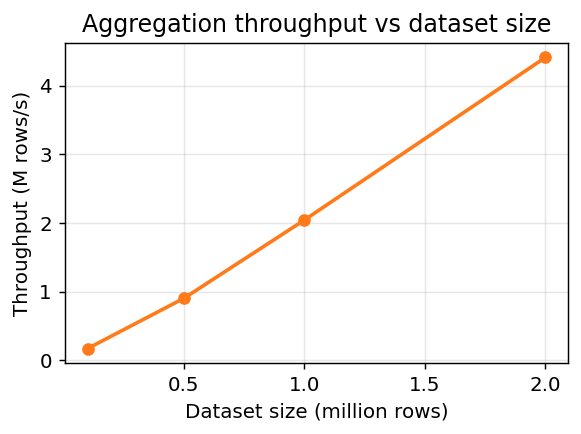
\includegraphics[width=0.95\columnwidth]{figures/throughput.png}
\caption{Aggregation throughput vs.\ dataset size. Fixed job overhead amortizes as
data grows.}
\label{fig:throughput}
\end{figure}

\textbf{Strong scaling.} Table~\ref{tab:scaling} and Fig.~\ref{fig:speedup} vary the
worker count for a fixed 2\,M-row job. Speed-up is modest (1.06$\times$ at two
cores) and \emph{regresses} at \code{local[4]} because the host has only two
physical cores and the job is overhead-bound, leaving little to parallelize. This
is the expected behavior for small jobs on small hardware and is revisited in
\S\ref{sec:threats}.

\begin{table}[t]
\centering
\caption{Strong scaling, fixed 2\,M-row job.}
\label{tab:scaling}
\small
\begin{tabular}{@{}crr@{}}
\toprule
\textbf{Workers (\code{local[k]})} & \textbf{Median time (s)} & \textbf{Speed-up} \\
\midrule
1 & 0.604 & 1.00$\times$ \\
2 & 0.570 & 1.06$\times$ \\
4 & 0.593 & 1.02$\times$ \\
\bottomrule
\end{tabular}
\end{table}

\begin{figure}[t]
\centering
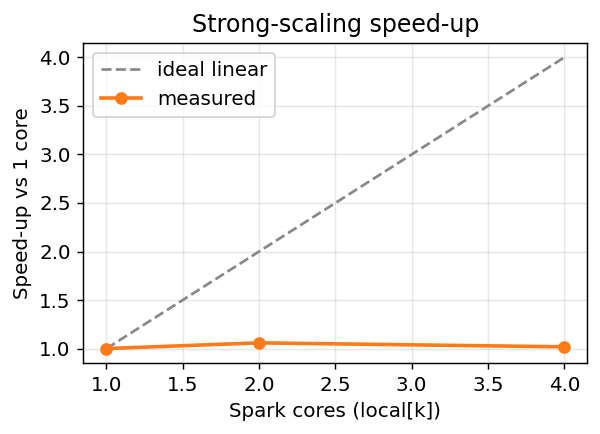
\includegraphics[width=0.95\columnwidth]{figures/speedup.png}
\caption{Measured speed-up vs.\ the linear ideal. The 2-core host bounds attainable
scaling.}
\label{fig:speedup}
\end{figure}

\textbf{Streaming ingestion.} A Structured Streaming query reading 100{,}000 events
across 40 newline-delimited JSON files with a stateful per-key count, executed via
\code{Trigger.AvailableNow}, completed in 8.34~s end-to-end---about
\textbf{11{,}989 events/s} including query planning and micro-batch scheduling.

\textbf{Auto-grader latency.} Fig.~\ref{fig:grader} and Table~\ref{tab:grader}
decompose interactive latency. Pure-Python challenges are graded in $\sim$1~ms.
Spark challenges incur a one-time JVM/session cold start of $\sim$3.5~s; a full
Spark grade (start + execute + check + teardown) completes in $\sim$8.6~s. The
warm-up dominates, which directly motivates the Spark~Connect warm-pool design
noted in \S\ref{sec:sandbox}: a shared session would remove the 3.5~s term from
every interaction.

\begin{table}[t]
\centering
\caption{Median auto-grader latency.}
\label{tab:grader}
\small
\begin{tabular}{@{}lr@{}}
\toprule
\textbf{Operation} & \textbf{Median latency} \\
\midrule
Python challenge (run + grade) & 1\,ms \\
Spark session cold start & 3{,}537\,ms \\
Spark challenge (end-to-end) & 8{,}569\,ms \\
\bottomrule
\end{tabular}
\end{table}

\begin{figure}[t]
\centering
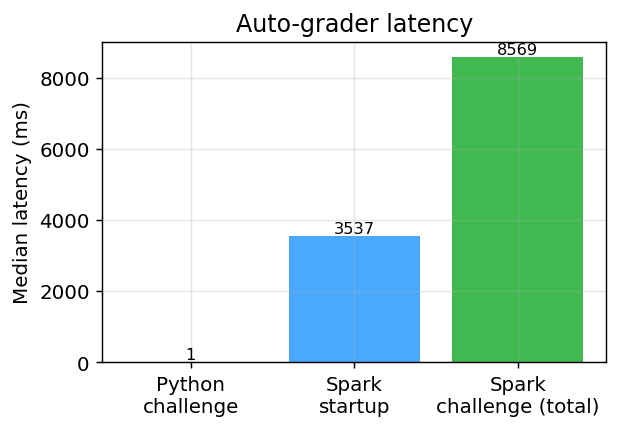
\includegraphics[width=0.95\columnwidth]{figures/grader_latency.png}
\caption{Auto-grader latency. The Spark cold start is the dominant, and removable,
cost.}
\label{fig:grader}
\end{figure}

\section{Threats to Validity}
\label{sec:threats}
Performance results are hardware-dependent and were gathered on a 2-vCPU host; the
flat throughput and limited speed-up reflect small, overhead-bound jobs rather than
a limitation of Spark, which scales to far larger data and clusters. We measure
\emph{system} performance, not learning outcomes; a user study with pre/post
assessments and engagement metrics is future work. Finally, the security analysis
is qualitative---the current sandbox targets a trusted, single-tenant demo, and
hostile-multi-tenant deployment requires the containerized isolation we describe.

\section{Future Work}
Planned extensions include: a warm Spark~Connect pool to remove cold-start latency;
persistent progress and authentication; a randomized-input grading mode to deter
hard-coding; a controlled study of learning gains and retention; and additional
tracks (Delta Lake, partitioning/shuffle tuning, and a capstone ETL project on a
real Kaggle dataset).

\section{Conclusion}
SparkQuest shows that a beginner can write and execute \emph{real} distributed Spark
code within minutes, with trustworthy automated feedback and game mechanics that
sustain progress. The system pairs a careful execution-and-grading design with a
complete, reproducible engineering pipeline---tests, CI, containerization, and
free live deployment. On a deliberately constrained host it sustains multi-million
row aggregation and $\sim$12k~events/s streaming, grades Python instantly, and
isolates a removable Spark cold start as its dominant interactive cost. The project
is open source and live; we hope it lowers the on-ramp to data engineering.

\begin{thebibliography}{99}
\small
\bibitem{zaharia2012rdd} M.~Zaharia \emph{et~al.}, ``Resilient distributed datasets:
A fault-tolerant abstraction for in-memory cluster computing,'' in \emph{Proc.
NSDI}, 2012.
\bibitem{zaharia2016spark} M.~Zaharia \emph{et~al.}, ``Apache Spark: A unified
engine for big data processing,'' \emph{Commun. ACM}, vol.~59, no.~11, pp.~56--65,
2016.
\bibitem{armbrust2015sparksql} M.~Armbrust \emph{et~al.}, ``Spark SQL: Relational
data processing in Spark,'' in \emph{Proc. ACM SIGMOD}, 2015.
\bibitem{armbrust2018streaming} M.~Armbrust \emph{et~al.}, ``Structured Streaming: A
declarative API for real-time applications in Apache Spark,'' in \emph{Proc. ACM
SIGMOD}, 2018.
\bibitem{dean2004mapreduce} J.~Dean and S.~Ghemawat, ``MapReduce: Simplified data
processing on large clusters,'' in \emph{Proc. OSDI}, 2004.
\bibitem{deterding2011gamification} S.~Deterding, D.~Dixon, R.~Khaled, and
L.~Nacke, ``From game design elements to gamefulness: Defining gamification,'' in
\emph{Proc. MindTrek}, 2011.
\bibitem{hamari2014gamification} J.~Hamari, J.~Koivisto, and H.~Sarsa, ``Does
gamification work? A literature review of empirical studies on gamification,'' in
\emph{Proc. HICSS}, 2014.
\bibitem{paiva2022automated} J.~C.~Paiva, J.~P.~Leal, and \'A.~Figueira,
``Automated assessment in computer science education: A state-of-the-art review,''
\emph{ACM Trans. Comput. Educ.}, vol.~22, no.~3, 2022.
\bibitem{edwards2004testing} S.~H.~Edwards, ``Using software testing to move
students from trial-and-error to reflection-in-action,'' in \emph{Proc. ACM
SIGCSE}, 2004.
\bibitem{wilcox2015automation} C.~Wilcox, ``The role of automation in undergraduate
computer science education,'' in \emph{Proc. ACM SIGCSE}, 2015.
\bibitem{kolling2010greenfoot} M.~K\"olling, ``The Greenfoot programming
environment,'' \emph{ACM Trans. Comput. Educ.}, vol.~10, no.~4, 2010.
\bibitem{ramirez2018fastapi} S.~Ram\'irez, ``FastAPI,'' 2018. [Online]. Available:
\url{https://fastapi.tiangolo.com}
\bibitem{biewald2020wandb} L.~Biewald, ``Experiment tracking with Weights and
Biases,'' 2020. [Online]. Available: \url{https://wandb.ai}
\end{thebibliography}

\end{document}
